\documentclass[12pt]{article}
\usepackage[english]{babel}
\usepackage[utf8x]{inputenc}
\usepackage[T1]{fontenc}
\usepackage{url}
\usepackage{scribe}
\usepackage{listings}
\usepackage{mathtools}
\usepackage{listings}
\usepackage{tikz}
\usepackage{xcolor}
\usepackage{amsmath}
\usepackage{float}

\lstdefinestyle{mystyle}{
    backgroundcolor=\color{backcolour},   
    commentstyle=\color{codegreen},
    keywordstyle=\color{magenta},
    numberstyle=\tiny\color{codegray},
    stringstyle=\color{codepurple},
    basicstyle=\ttfamily\footnotesize,
    breakatwhitespace=false,         
    breaklines=true,                 
    captionpos=b,                    
    keepspaces=true,                 
    numbers=left,                    
    numbersep=5pt,                  
    showspaces=false,                
    showstringspaces=false,
    showtabs=false,                  
    tabsize=2
}

\tikzstyle{data} = [circle, minimum size = 3 cm,text centered, draw=black, thick, fill=red!30, text=white]
\tikzstyle{model} = [rectangle, minimum width=3cm, minimum height=3cm, text centered, draw=black, fill=orange!30]
\tikzstyle{arrow} = [thick,->,>=stealth]
\tikzstyle{outp} = [rectangle, rounded corners, minimum width=3cm, minimum height=3cm,text centered, draw=black, fill=green!30]

\Scribe{Aditya, Jay, Soham \& Sooraj}
\Lecturer{Abir De}
\LectureNumber{16}
\LectureDate{17 March 2023}

\LectureTitle{Gaussian Processes}

\lstset{style=mystyle}

\begin{document}
	\MakeScribeTop

%#############################################################
%#############################################################
%#############################################################
%#############################################################

% This is some warmup discussion before the first section.

% \section{Here's a section header}

% Here's some more text.
% % Here's a citation~\cite{Kar84a}.

% \subsection{Here's a subsection}

% You might like to put use subsectioning these too.  An alternate way to put in a small subheading for a paragraph is to use the \begin{verbatim} \paragraph \end{verbatim} command.  For example:

% \paragraph{A remembrance by Dantzig.}  The early days were full of intense excitement. Scientists, free at last from war-time pressures, entered the post-war period hungry for new areas of research. The computer came on the scene at just the right time. Economists and mathematicians were intrigued with the possibility that the fundamental problem of optimal allocation of scarce resources could be numerically solved. Not too long after my first meeting with Tucker there was a meeting of the Econometric Society in Wisconsin attended by well-known statisticians and mathematicians like Hotelling and von Neumann, and economists like Koopmans. I was a young unknown and I remember how frightened I was at the idea of presenting for the first time to such a distinguished audience, the concept of linear programming.



% \section{Math stuff}

% Please make an effort to typeset things nicely.  There are quite a few macros in the lpsdp.sty file.  Below are illustrated how to do some basic things; please study the \LaTeX\ carefully.

% Here's a typical LP in standard/equational form, with an equation number on one of the constraints.
% \begin{gather}
%     \min \quad c^\top x                       \nonumber\\
%     \begin{aligned}
%         \text{s.t.} \quad   Ax &= b           \nonumber\\
%                              x &\geq 0       \label{eqn:nonnegative}
%     \end{aligned}
% \end{gather}

% \noindent Here's a reference to the~\eqref{eqn:nonnegative} nonnegativity constraint.  Some more LPs:

% \begin{gather*}
%     \min \quad 3x_1 - 5x_2 \\
%     \begin{aligned}
%         \text{s.t.} \quad   x_1 + 2x_2 &\leq 6\\
%                             2x_1 + x_2 &\leq 6\\
%                             2x_1 + 2x_2 &\geq 7\\
%                             x_1,x_2 &\geq 0
%     \end{aligned}
% \end{gather*}

% \begin{alignat*}{3}
%     \text{minimize}&   \quad & 3x_1 - 5x_2 + 2x_3 - x_4&       & &\\
%     \text{subject to}& \quad & x_1 + 2x_2 - 4x_3 + x_4 &\leq 6 & &\\
%                            & & -x_1 + 3x_2 - x_3 - x_4 &\geq 7 & &\\
%                            & & x_i &\geq 0  & &\quad \forall i = 1\dots 4
% \end{alignat*}

% \begin{align}
%     & \min_{\varepsilon^{up}, \varepsilon^{dw}, \beta}  &&  \sum_{i \in Observations} {\varepsilon^{up}}_i + {\varepsilon^{dw}}_i  && \notag \\
%     & \text{subject to}     &&  {\varepsilon^{up}}i \geq + y_i - \sum{j \in Candidates} \beta_j x_{i,j} && \forall i \in Observations \notag \\
%     &                       &&  {\varepsilon^{dw}}i \geq - y_i + \sum{j \in Candidates} \beta_j x_{i,j} && \forall i \in Observations \notag \\
%     &                       &&  {\varepsilon^{up}}_i, {\varepsilon^{dw}}_i \geq 0 && \forall i \in Observations \notag \\
% \end{align}

% \begin{alignat*}{4}
% z_k(x) \ = \ & \min_{y_k}        &       &  f_k^T y_k &&                  \notag \\
%              & \text{subject to} & \quad &  D_k y_k   &&  = d_k - B_k x  \notag \\
%              &                   &       &  y_k       && \geq 0          \notag \\
% \end{alignat*}

% Huge LP's:

% \begin{align}
%     & \min_{x, y_k}     &&  c^T x && + f_1^T y_1 && + \dots && + f_n^T y_n  &&  \notag \\
%     & \text{subject to} &&  Ax    &&             &&         &&              && = b \notag \\
%     &                   &&  B_1 x && + D_1 y_1   &&         &&              && = d_1 \notag \\
%     &                   &&  \dots &&             &&  \dots  &&              &&       \notag \\
%     &                   &&  B_n x &&             &&         && + D_n y_n    && = d_n \notag \\
%     &                   &&   x,   &&     y_1,    &&         &&       y_n    && \geq 0 \notag \\
% \end{align}


% Let's do some matrices:
% \[
% \begin{pmatrix}
%     1 & \rho & \rho\\
%     \rho & 1 & \rho\\
%     \rho & \rho & 1\\
% \end{pmatrix},
% \quad \text{or alternately,} \quad
% \begin{bmatrix}
%     1 & 2 \\
%     3 & 4 \\
% \end{bmatrix}.
% \]
% More generically:
% \[
%     A = \begin{bmatrix}
%             \vrule & \vrule & & \vrule\\
%             A_{1} & A_{2} & \cdots & A_{n} \\
%             \vrule & \vrule & & \vrule
%         \end{bmatrix}
%       = \begin{bmatrix}
%             \text{---} & a_1 & \text{---} \\
%             \text{---} & a_1 & \text{---} \\
%                        & \vdots &  \\
%             \text{---} & a_n & \text{---} 
%         \end{bmatrix}
% \]


% Here's some more random typesetting: 
% \begin{itemize}
% \item ``PTIME vs. NP, where the former means time $\poly(n)$'';
% \item $\wt{O}(f(x)) \text{ is } f(x) \cdot \polylog(f(x))$;
% \item $\displaystyle 
%         g(x) = \begin{cases}
%                    \sin(2\theta) & \text{if $\theta \leq \pi$,}\\
%                    \max\{\cos^2\theta, \tfrac13\} & \text{if $\theta > \pi$.}
%                \end{cases}
%       $
% \end{itemize}
% Please don't write $max(A)$ when you mean $\max(A)$, or $log(n)$ when you mean $\log(n)$, or "quotes" when you mean ``quotes''.

% \

% More equations:

% $\max \Big\{ \sum_{i \in Observations} \Big( y_i - \sum_{j \in Candidates} \beta_j x_{i,j} \Big) ^2 \Big\}$

% $\max\Bigg\{ \sum_{i \in Observations} \Big| y_i - \sum_{j \in Candidates} \beta_j x_{i,j} \Big| \Bigg\}$

% A theorem and a proof:
% \begin{theorem} $(a+b)^2 = a^2 + 2ab + b^2$.
% \end{theorem}
% \begin{proof}
% Let for the reader.
% \end{proof}

% \bigskip

% Here's what to do if your proof ends on an equation:
% \begin{proof}
% It's easy:
% \[
%     (a+b)^2 = (a+b)(a+b) = (a+b)a + (a+b)b = a^2 + ba + ab + b^2 = a^2 + 2ab + b^2 \qedhere
% \]
% \end{proof}

% And a lemma without proof:
% \begin{lemma}
% Suppose numbers exist, then $(a+b)^2 = a^2 + 2ab + b^2$.
% \end{lemma}

% You can do a few others:
% \begin{example}
% Suppose numbers exist, then $(a+b)^2 = a^2 + 2ab + b^2$.
% \end{example}
% \begin{conjecture}
% Suppose numbers exist, then $(a+b)^2 = a^2 + 2ab + b^2$.
% \end{conjecture}
% \begin{definition}
% Suppose numbers exist, then $(a+b)^2 = a^2 + 2ab + b^2$.
% \end{definition}
% \begin{observation}
% Suppose numbers exist, then $(a+b)^2 = a^2 + 2ab + b^2$.
% \end{observation}
% \begin{remark}
% Suppose numbers exist, then $(a+b)^2 = a^2 + 2ab + b^2$.
% \end{remark}
% \begin{claim}
% Suppose numbers exist, then $(a+b)^2 = a^2 + 2ab + b^2$.
% \end{claim}



% Please insert figures liberally.  It's probably best if ``vector graphics'' are in pdf or png format, and ``bitmap graphics'' are in jpg format, but lots formats are supported.  There's a macro defined to make things easy.  Inkscape is a pretty reasonable, free program in which to draw figures.
 
% %%%%%%%% FIGURES
% % first parameter is a real number which is the scale factor; 
% % second is the file name; 
% % third is caption; 
% % fourth gives the LaTeX label for future \ref
% \myfig{.375}{example-figure.pdf}{The region $g_1 > 0, g_2 > -\tfrac{\rho}{\sqrt{1-\rho^2}}g_1$.}{fig:my-example}

% Once you've inserted it, you can refer to it as Figure~\ref{fig:my-example}.\\

% Here there is an example of some code
% \begin{lstlisting}[language=Julia]
% using JuMP, GLPK

% function production_model()
%     # Define an optimization model
%     m = Model(with_optimizer(GLPK.Optimizer))
    
%     # Variables
%     @variable(m, x[i in 1:2] >= 0)
    
%     # Constraints
%     @constraint(m, 2*x[1] + x[2] <= 4)
%     @constraint(m, x[1] + 2*x[2] <= 4)
    
%     # Objective function
%     @objective(m, Max, 4*x[1] + 3*x[3])
    
%     # Solve the model
%     optimize!(m)
    
%     return objective_value(m)
% end
% \end{lstlisting}
% Finally, if you have citations, see the commented-out stuff in the \LaTeX~here.

% \

% My farourive Optimization books are \cite{bertsimas1997introduction} \cite{boyd2004convex} \cite{wolsey2014integer}. You should add bibliographical notes in the \textbf{BibTex}: \textit{mybib.bib} file. Its good to grab these notes from Google scholar citations.

% %%%%%%%%%%% If you don't have citations then comment the lines below:
% %

% Till now, we haven't discussed minimization of \textbf{Supervised Learning Algorithms yet}. In this lecture, we cover the optimisation technique \textbf{Gradient Descent}; the working of the algorithm, the cause of stochastic behaviour of gradient descent and how to utilise this stochastic nature to our advantage. We also see applications of gradient descent in an upcoming technology known as \textit{MLaaS} (\textit{M}achine \textit{L}earning \textit{a}s \textit{a} \textit{S}ervice). This lecture is mainly theoretical in nature where many concepts are just introduced at a very high level without getting into the Maths and detailed theory involved.
Till now we had studied about kernels and their properties. In the last lecture, we learned about Gaussian Processes(GP).

\section{Recap of the last lecture}
Let's begin with a brief introduction to Gaussian processes.\\
\\
Gaussian Processes are a class of probabilistic models that can be used for supervised machine-learning tasks such as regression and classification. GPs are a non-parametric approach, meaning they do not assume any particular functional form for the relationship between the inputs and outputs.\\
\\
In a GP, a function is modeled as a probability distribution over functions. This distribution is defined by a mean function and a covariance function. The mean function specifies the expected value of the function at each input point, while the covariance function specifies how much the function values at different input points are correlated.\\
\\
During training, the GP is fitted to the training data by adjusting the hyper-parameters to maximize the likelihood of the observed data. Once the GP is trained, it can be used to make predictions for new inputs by computing the posterior distribution over functions given the observed data.\\

\section{Gaussian Processes and Multivariate Gaussian Distribution}
A multivariate Gaussian distribution is a probability distribution that describes the joint probability distribution of a set of random variables that are normally distributed. It is an extrapolation of the univariate Gaussian distribution to higher dimensions, where the mean vector and covariance matrix fully specify the distribution.\\
\\
The multivariate Gaussian distribution is widely used in statistics, machine learning, and many other fields, due to its flexibility and tractability. It is used in applications such as clustering, classification, regression and data analysis among others.\\

\subsection{2-dimensional Gaussian Distribution}

\begin{equation}
    y \sim \mathcal{N}(\mu,\Sigma)
\end{equation}
where $y$ and $\mu$ are two-dimensional vectors and $\Sigma$ is $2$x$2$ matrix given by:
\begin{align}
    \Sigma &= \begin{bmatrix}
            \Sigma_{AA} & \Sigma_{AB}\\
            \Sigma_{BA} & \Sigma_{BB}\\
        \end{bmatrix}
\end{align}
\\
where $\Sigma_{aa}$ represents the variance of $a$ and $\Sigma_{ab}$ is a co-variance of $a$ and $b$.\\
\begin{equation}
    f(x) = \frac{1}{\sqrt{2\pi|\Sigma|^2}}e^{-\frac{(x-\mu)^T\Sigma^{-1}(x-\mu)}{2}}
\end{equation}
\subsection{Conditional Gaussian Distribution}
 We have two random variables $X$ and $Y$, and we know that $Y$ is dependent on $X$, then the conditional distribution of $Y$ given $X$ can be represented as a Gaussian distribution.\\
 \begin{equation}
      Y_A|Y_B \sim \mathcal{N}(\mu'_A,\Sigma_{A|B})
 \end{equation}

 \noindent
 Now, let's see the effect of conditioning on the mean of a distribution:\\
If we observe one variable,\\
 let's say $Y_B$ = $Y_0$, then $Y_B$ is a distribution with mean $Y_0$ and variance 0. \\
 Start with the intuition:  \\
 
 
 \begin{equation}
     \mu'_A = \mu_A + \Sigma_{AB}\Sigma_{BB}^{-1}(Y_0-\mu_B)
 \end{equation}
\textbf{Verification of our intuition:}
\begin{itemize}
    \item If $Y_B = \mu_B$, then the mean of $Y_A$ won't change which can be seen in the equation. $Y_0 = \mu_B$ then $\mu'_A = \mu_A + 0$.
    \item Substituting A with B yields, $\mu'_B = \mu_B + \Sigma_{BB}\Sigma_{BB}^{-1}(Y_0-\mu_B)=Y_0$ 
    \item If co-variance of $Y_A$ and $Y_B$ is zero, then after observation mean of $Y_A$ doesn't change.\\
    $\Sigma_{AB}=0$, so $\mu'_A = \mu_A $
    \item If $\Sigma_{BB}$ is very large, it means that there is a large variation in $Y_B$. Hence, we shouldn't rely on the observed value of $Y_B$  and thus, the mean remains unaffected.
    \item Now $\Sigma_{BB}\rightarrow0$ which means that $Y_B$ is a constant then $(Y_B-\mu_B) \rightarrow 0$
\end{itemize}
So, we have to calculate the limit for $\mu'_A$,
\begin{equation}
    \lim_{\Sigma_{BB}\rightarrow0}(\mu'_{A}) = \mu_A + \lim_{\Sigma_{BB}\rightarrow0}[\Sigma_{AB}\Sigma_{BB}^{-1}(Y_0-\mu_B)]
\end{equation}
\newpage
\noindent
\textbf{Calculating the limit:}

\begin{equation}
    \textbf{L} = \lim_{\Sigma_{BB}\rightarrow0}[\Sigma_{AB}\Sigma_{BB}^{-1}(Y_0-\mu_B)]
\end{equation}
    
\noindent
where,
$\Sigma_{AB}$ = \E[$(Y_A-\mu_A)(Y_B-\mu_B)$],  $\Sigma_{BB}$ = \E[$(Y_B-\mu_B)^2$].\\

\noindent
Since variance is tending towards zero, $(Y_B-\mu_B)$ can be assumed as constant.
\begin{equation}
      \textbf{L} = \lim_{\Sigma_{BB}\rightarrow0}\frac{(Y_B-\mu_B)^2\E[Y_A-\mu_A]}{(Y_B-\mu_B)^2}
\end{equation}
\begin{equation}
= \lim_{\Sigma_{BB}\rightarrow0}\E[Y_A-\mu_A] = 0
\end{equation}
so,
\begin{equation}
    \lim_{\Sigma_{BB}\rightarrow0}(\mu'_A) = \mu_A + 0 = \mu_A
\end{equation}

\noindent
Now that we have observed the effect of conditioning on the mean of a distribution, we proceed with the variance of $Y_A|Y_B$. Intuitively, one can guess the variance to be the following:
\begin{equation}
    \Sigma_{A|B}= \Sigma_{AA}-\Sigma_{AB}\Sigma_{BB}^{-1}\Sigma_{BA}
\end{equation}
\textbf{Verification of our intuition:}

\begin{itemize}
    \item If $A=B$, then the value of variance will be: \\
    \begin{equation}
       \Sigma_{B|B} = \Sigma_{BB}-\Sigma_{BB}\Sigma_{BB}^{-1}\Sigma_{BB}    
    \end{equation}
    
    \begin{equation}
        = \Sigma_{BB}-\Sigma_{BB}I = 0
    \end{equation}
    
    Hence, we obtain  $\Sigma_{B|B} = 0$.
    
    \item When $\Sigma_{BB}\rightarrow \infty$:
    \begin{equation}
        \Sigma_{A|B}= \lim_{\Sigma_{BB}\rightarrow \infty} (\Sigma_{AA}-\Sigma_{AB}\Sigma_{BB}^{-1}\Sigma_{BA})
    \end{equation}
    \end{itemize}
    \noindent
    Now, we need to calculate the limit for $\Sigma_{A|B}$,  \\
    \textbf{Calculating the limit:}
    \begin{equation}
        \textbf{L} = \lim_{\Sigma_{BB}\rightarrow \infty}(\Sigma_{AA}-\Sigma_{AB}\Sigma_{BB}^{-1}\Sigma_{BA})
    \end{equation}
    \noindent
    where,
    $\Sigma_{AB}$ = \E[$(Y_A-\mu_A)(Y_B-\mu_B)$]= $\Sigma_{BA}$,  $\Sigma_{BB}$ = \E[$(Y_B-\mu_B)^2$].\\
    \begin{equation}
      \textbf{L} = \lim_{(Y_{B}-\mu_{B})^2\rightarrow \infty}\Biggl(\E[(Y_A-\mu_A)^2]-\frac{(\E[(Y_A-\mu_A)(Y_B-\mu_B)])^2}{\E[(Y_B-\mu_B)^2]}\Biggl)
    \end{equation}
    \noindent
    As $\E[(Y_B-\mu_B)^2]$ becomes arbitrarily large, we can conclude that:
\begin{equation}
    \textbf{L} = \lim_{(Y_{B}-\mu_{B})^2\rightarrow \infty}\Biggl(\E[(Y_A-\mu_A)^2]-\frac{(\E[(Y_A-\mu_A)(Y_B-\mu_B)])^2}{\E[(Y_B-\mu_B)^2]}\Biggl)=\E[(Y_A-\mu_A)^2]=\Sigma_{AA}
\end{equation}
\noindent
One more argument that can be made in the favour of the above result is that since $\Sigma_{BB}$ is arbitrarily large $Y_{B}$ is effectively a noise term and the distribution of $Y_{A}|Y_{B}$ is identical to that of $Y_{A}$.
\noindent
Thus, we have modeled the bi-variate Gaussian distribution in the following manner:
 \begin{equation}
      Y_A|Y_B \sim \mathcal{N}\Biggl(\mu_A + \Sigma_{AB}\Sigma_{BB}^{-1}(Y_0-\mu_B),\Sigma_{AA}-\Sigma_{AB}\Sigma_{BB}^{-1}\Sigma_{BA}\Biggl)
 \end{equation}
 \noindent
 Following is a plot of the joint, marginal and conditional distribution for a bivariate gaussian function which has been discussed above. 
\begin{figure}[H]
     \centering
     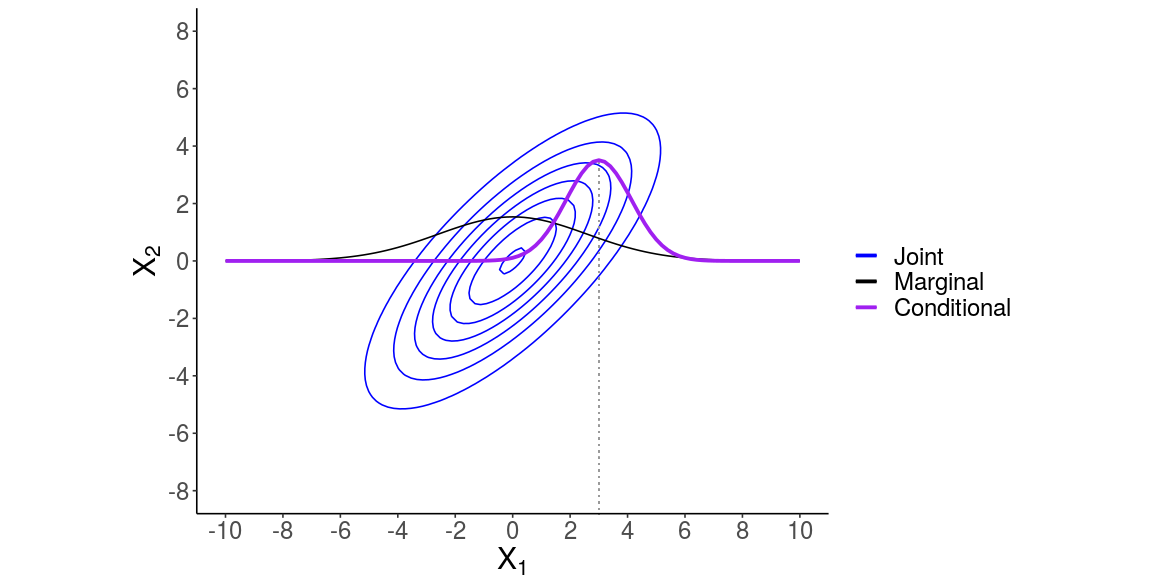
\includegraphics[scale=0.5]{gaussian_img.png}
     \caption{Joint, Marginal and Conditional Distribution for bivariate Gaussian distribution \\ \hfill \tiny{\textit{source: {https://fabiandablander.com/statistics/Two-Properties.html}}}}
     \label{fig:my_label}
 \end{figure}
\noindent 
We have used an extremely intuitive approach to modeling the bivariate Gaussian distribution, a more complete and rigorous derivation of the same can be found at \url{https://fabiandablander.com/statistics/Two-Properties.html}.






            


\end{document}